\documentclass[noback,noborder,portrait,twocolumn]{cuposter}

%%\documentclass[noback,portrait]{cuposter}
%% To make a poster in portrait, use the "portrait" option to
%% documentclass as shown above.

\usepackage{mathptmx}
\usepackage{xspace}
\usepackage{amsmath}
\usepackage{pifont}
\usepackage{psfrag}

\usepackage{graphicx}
%% \usepackage{subcaption}
\usepackage{wrapfig}

\usepackage{hyperref}
\usepackage{xcolor}
\usepackage[normalem]{ulem}

\usepackage{../macros}

\useunder{\uline}{\ulined}{}%
\DeclareUrlCommand{\bulurl}{\def\UrlFont{\ttfamily\color{blue}\ulined}}


\begin{document}

%% Not needed for most posters.
%%\renewcommand{\poster@ancimage}{/tmp/empty.ps}
%% \newcommand{\don}{\ensuremath{d_{\textsc{ON}}}}
%% \newcommand{\doff}{\ensuremath{d_{\textsc{OFF}}}}
%% \newcommand{\dsoma}{\ensuremath{d_{\textsc{SOMA}}} \xspace}
%% \newcommand{\um}{\ensuremath{\mu \text{m}}\xspace}
%% \newcommand{\dmin}{d$_{\textup{min}}$\xspace}

\newcommand{\figspace}{\vskip 20pt plus 5pt minus 5pt}
\newcommand{\captionspace}{\vskip 10pt plus 5pt minus 5pt}

%%%NOTE: \linewidth IS THE CORRECT MACRO FOR SPECIFYING THE LENGTH OF COLUMNS

\newcounter{figcounter}
\newcommand{\getIncFigcounter}{\stepcounter{figcounter}\thefigcounter}
\title{\sciwms{}: Python Based Web Mapping Service For Visualizing Geospatial Data}

\newcounter{tablecounter}
\newcommand{\getIncTablecounter}{\stepcounter{tablecounter}\thetablecounter}

%%\subtitle{The poster subtitle here}
\author{Brandon A. Mayer$^{1,2}$, Brian McKenna$^{2}$, Dave A. Foster$^{2}$, Kelly Knee$^{2}$}
\address{Brown University, Providence RI, USA$^{1}$; RPS-ASA, South Kingston RI, USA$^{2}$}
%% \address{$^1$University of Cambridge and University of Edinburgh, UK;
%%   $^2$University of Lancaster, UK; $^3$Northwestern University, USA.}

\makeposter

\section{Introduction}
\begin{itemize}
  \item \sciwms{} is an open-source Python implementation of the
    \href{http://www.opengeospatial.org/standards/wms}{\color{blue}\ogc{}
      \wms{}} (Web Mapping Service) API for
    \href{http://cfconventions.org/}{\color{blue}CF-Compliant}
    coastal, atmospheric, climate and weather data with support for
    structured and unstructured topologies
  
  \item Deployed within the
    \href{http://www.ioos.noaa.gov/modeling/testbed.html}{{\color{blue}IOOS-COMT}}
    project scope for qualitatively assessing society-critical
    atmostpheric and oceanagraphic model and forcasting data
    including: forecasting, risk assessment, model comparison,
    algorithmic/parameter selection
    
  \item Achieves real-time visualization of
    externally hosted CF-Compliant data

  \item Can visualize data registered to structured or unstructured
    grids by adhering to
    \href{https://github.com/ugrid-conventions/ugrid-conventions/blob/v0.9.0/ugrid-conventions.md}{\color{blue}CF-UGRID
      Conventions}

  \item Abstracts a dataset into two objects: a topology
      and corresponding model data.
    
  \item Topologies are stored locally for efficient spatial queries

  \item Model data is hosted externally, subsets of which are
    downloaded and rendered per request

  \item Supports arbitrary cartographic projections 
  
  \item Source code is available at {\color{blue}
    \url{https://github.com/brandonmayer/sci-wms/tree/testbed}}
    
  \item Deployed for COMT-IOOS at {\color{blue}
    \url{http://testbedwww.sura.org/explorer/}}
\end{itemize}


\section{Architecture Overview}

%% \begin{minipage}[r]{\linewidth}
%%   \centering
%%   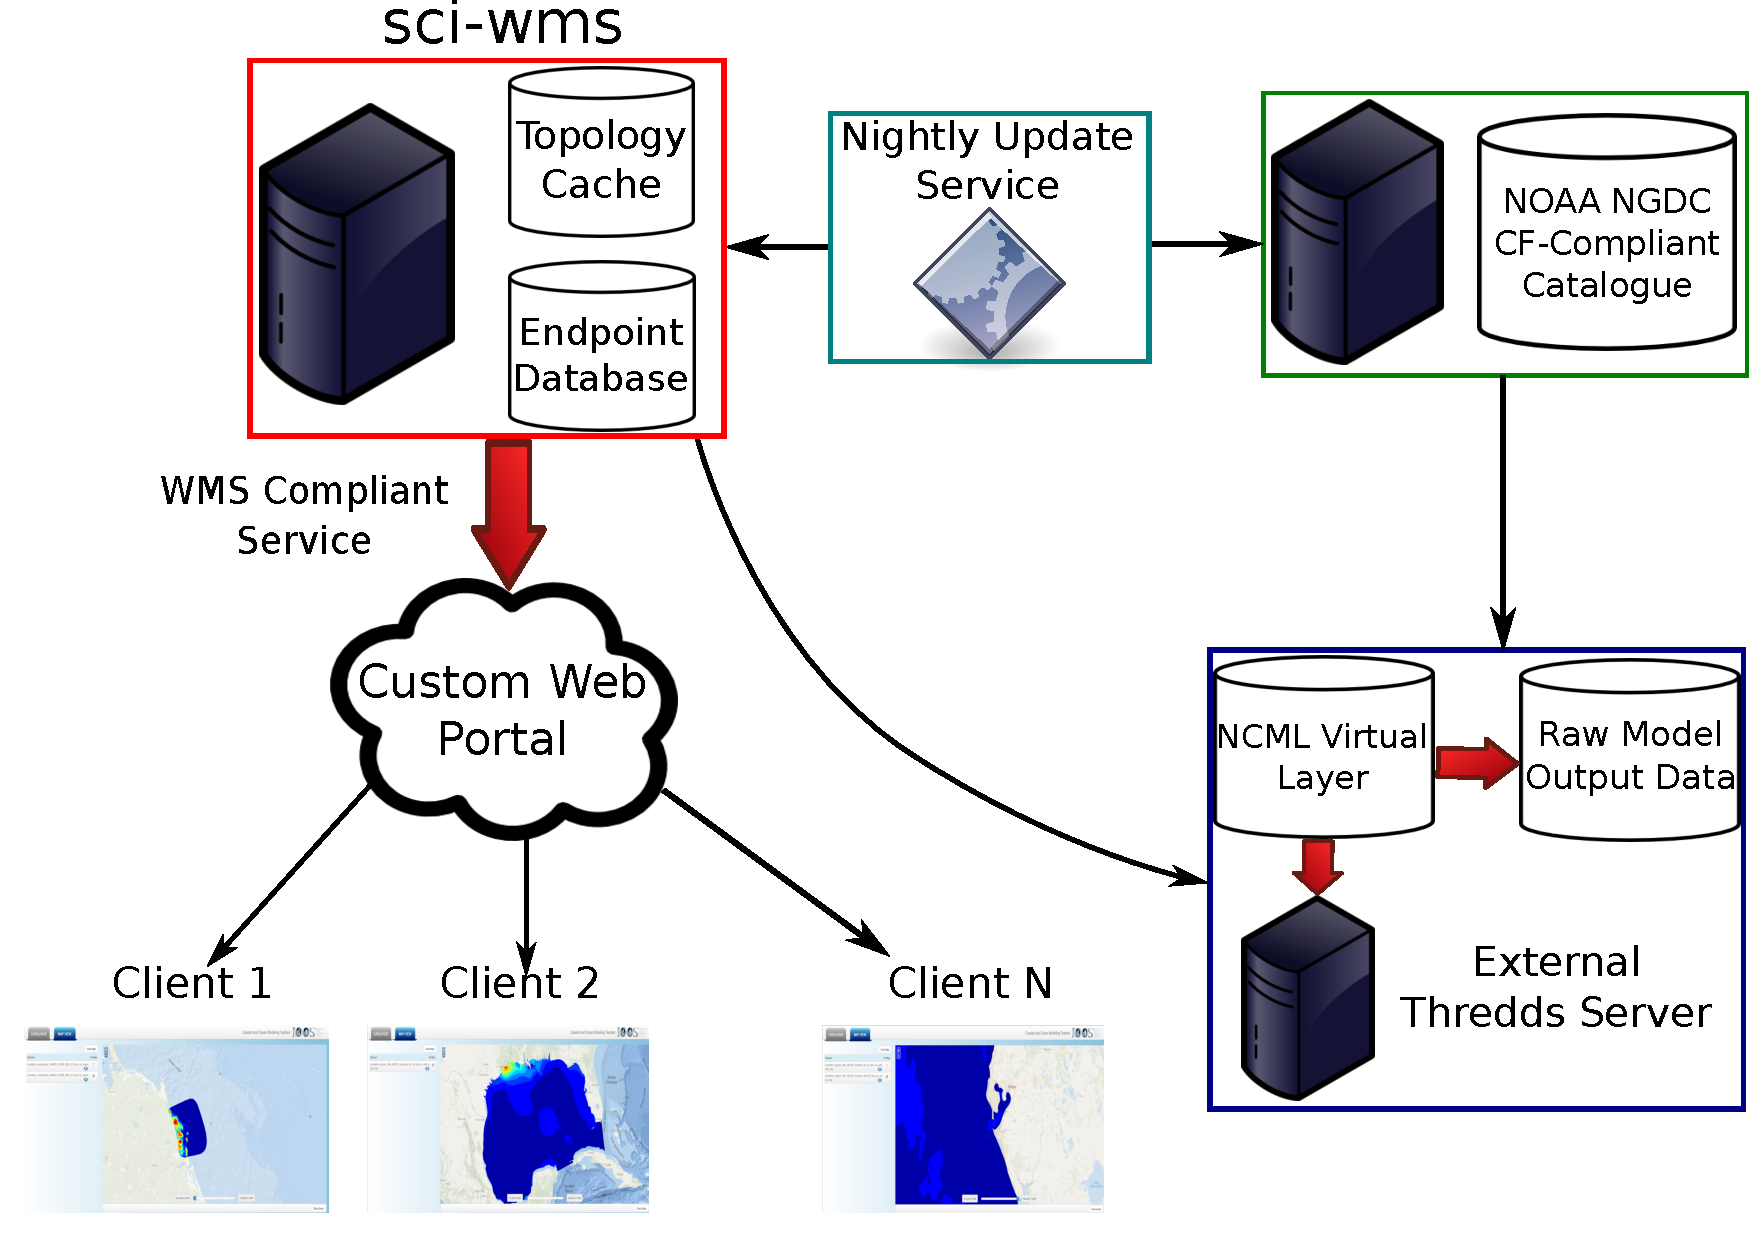
\includegraphics[width=0.45\linewidth]{../figs/overview.pdf}
%%   \captionspace{}
%%   \textbf{Figure \getIncFigcounter{}}: \textit{Overview of the \sciwms{} architecture within the scope of the U.S. \ioos{} \comt{} project.}
%% \end{minipage}

%% \figspace{}

%% \begin{minipage}[t]{\linewidth}
%%   \centering
%%   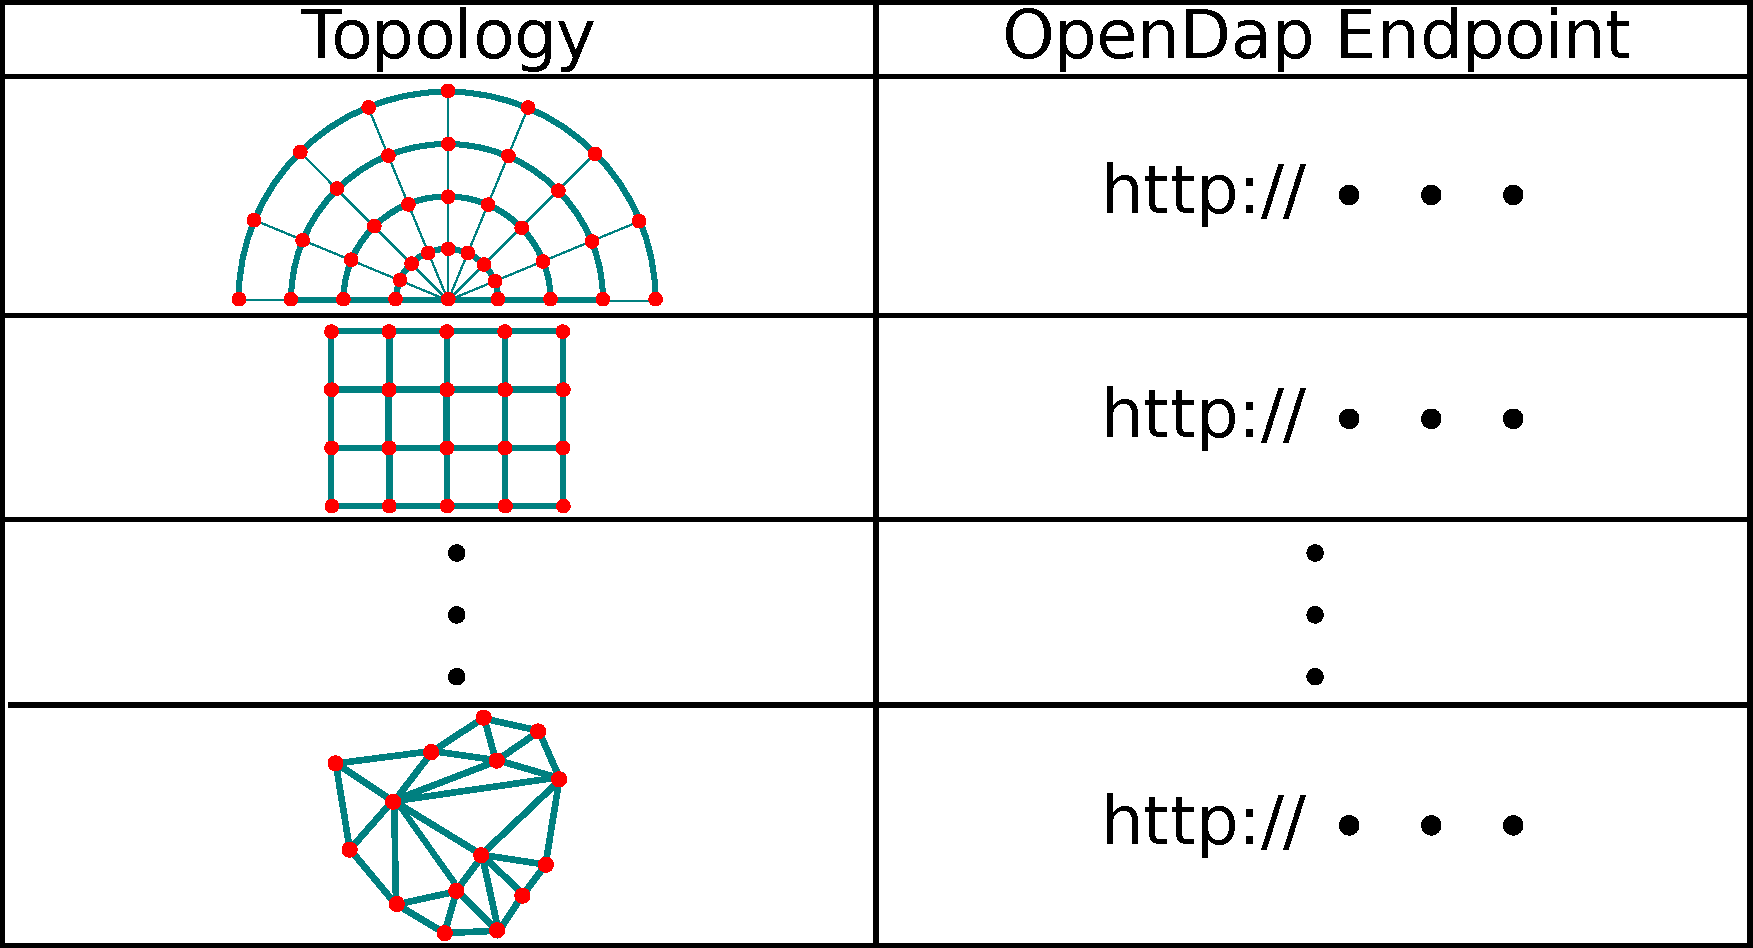
\includegraphics[width=\linewidth]{../figs/sciwms_db_topology_endpoints.pdf}
%%   \textbf{Figure \getIncFigcounter{}}: \textit{Topology and endpoint data store. Topologies are classified as either \cgrid{} or \ugrid{} for efficient geospatial queries and remote model data access.}
%% \end{minipage}

\begin{minipage}[t]{0.49\linewidth}
  \centering
  %% 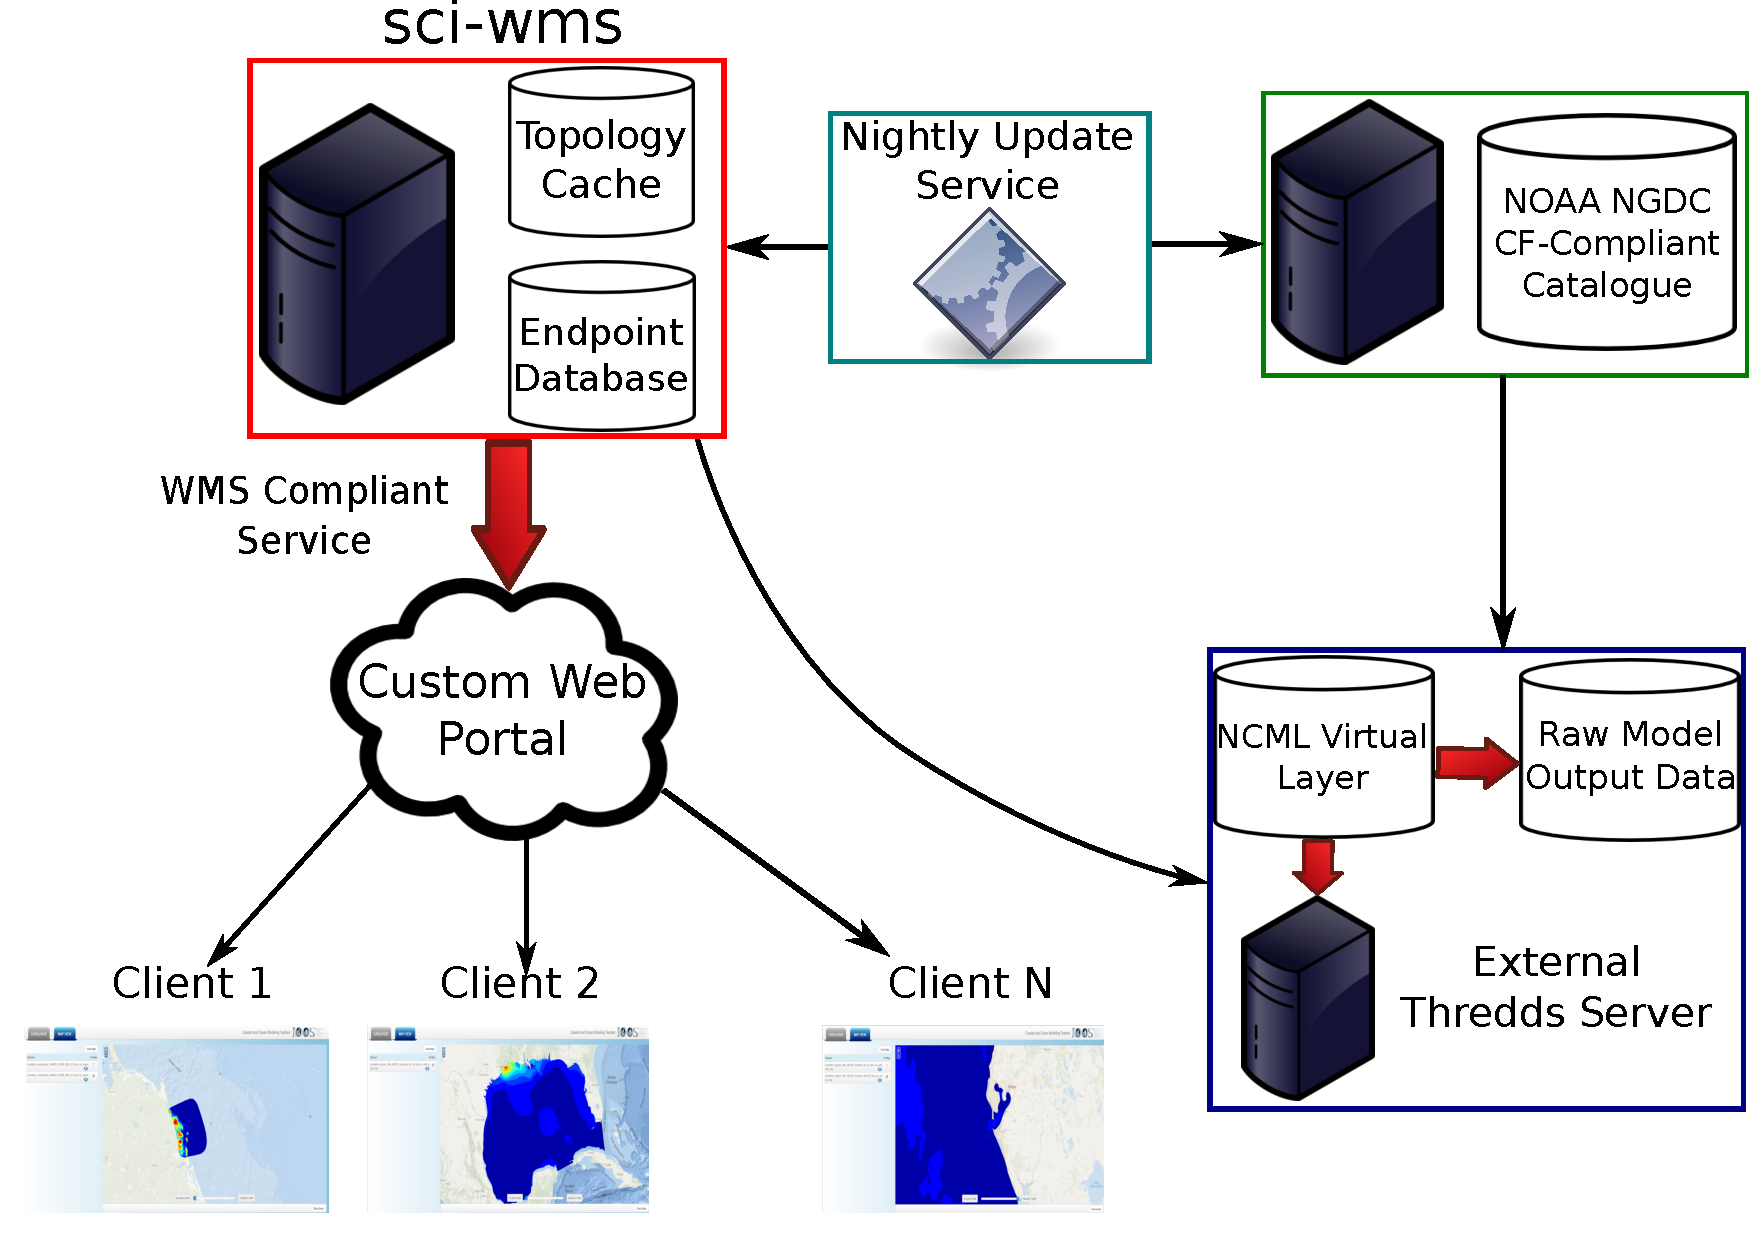
\includegraphics[width=\linewidth]{../figs/overview.pdf}
  \includegraphics[width=\linewidth]{../figs/sciwms_overview_v2.pdf}
  \captionspace{}
  \textbf{Figure \getIncFigcounter{}}: \textit{Overview of the \sciwms{} architecture within the scope of the U.S. \ioos{} \comt{} project.}
\end{minipage}
\begin{minipage}[t]{0.49\linewidth}
  \centering
  %% \raisebox{0.15\height}{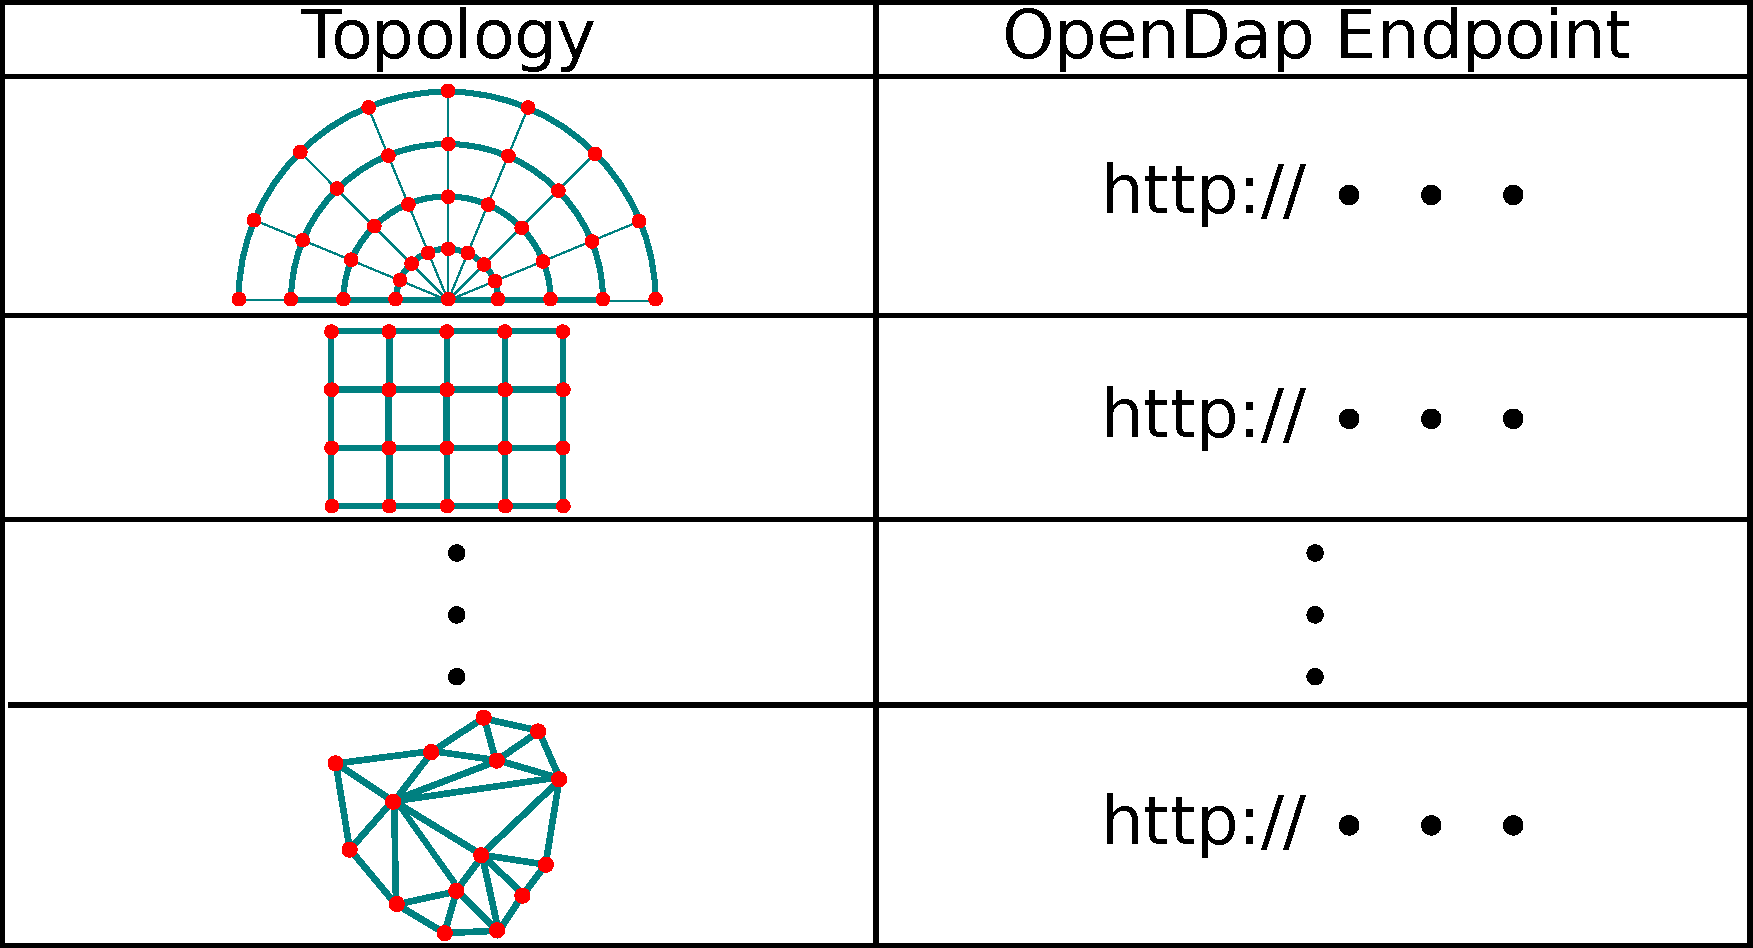
\includegraphics[width=\linewidth]{../figs/sciwms_db_topology_endpoints.pdf}}
  \includegraphics[width=\linewidth]{../figs/sciwms_book_db_topology_endpoint_chart}
  \textbf{Figure \getIncFigcounter{}}: \textit{Topology and endpoint data store. Topologies are classified as either \cgrid{} or \ugrid{} for efficient geospatial queries and remote model data access.}
\end{minipage}


\figspace{}

\begin{itemize}
    \item Unstructured grid locations are cached using R-Trees
      \begin{itemize}
        \item Fast queries for lat/lon coordinates lying within
          current view for a \wms{} \getMap{} request
          
        \item Fast K-nearest point lookups for \getFeatureInfo{} requests.
      \end{itemize}
\end{itemize}

\section{\wms{} Extensions}

While \sciwms{} is fully complient with the \ogc{} \wms{}
specification, \sciwms{} supports extensions to augment and simplify
the basic \wms{} API for rapid front end UI development

\begin{itemize}
  \item Query and return list of all available datasets and layers via
    json(p)

  \item Return requests for subsets (spatial/temporal) of raw model
    data as json(p)
    
  \item Responsds to requests for all available styles and colormaps
    in json(p) format
    
  \item Can generate and serve color-ramp previews
\end{itemize}

\section{Examples}
\begin{minipage}[t]{\linewidth}
  \centering
  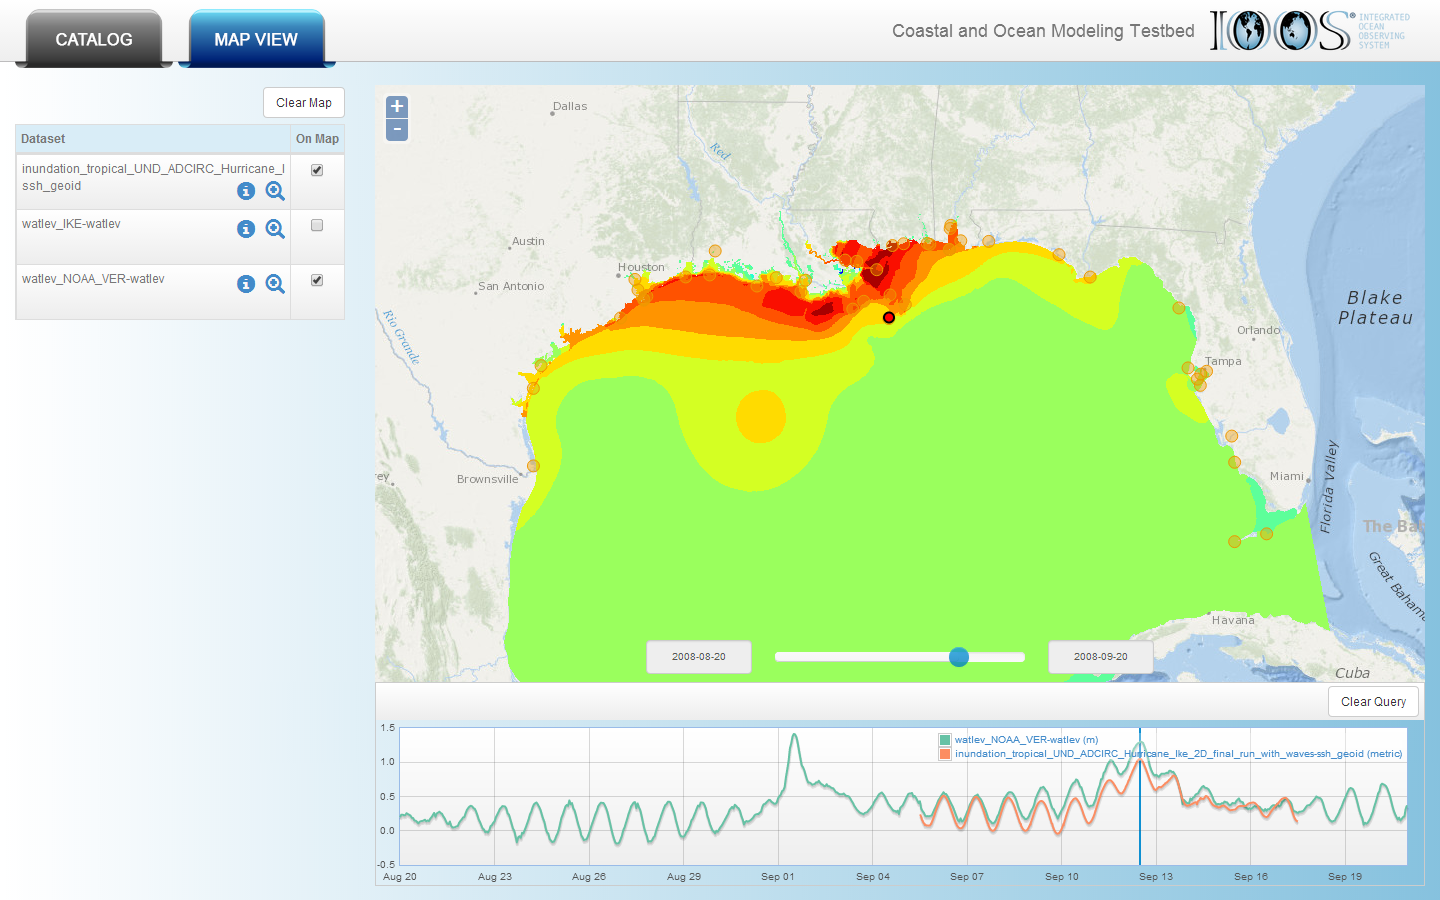
\includegraphics[width=\linewidth]{../figs/SciWMS_ModelObsComparison}
  \textbf{Figure \getIncFigcounter{}}: \textit{Comparison of ADCIRC
    (unstructured topology) model results with observed water levels
    in the Northern Gulf of Mexico for Hurricane Ike. Verified
    observed water levels are from NOAA's Station 8760922 (red dot on
    map). The map shows modeled water levels (in meters above the
    geoid) at the peak of the storm in southern Louisiana. The time
    series plot shows both the modeled (green) and observed (orange)
    water levels. The vertical blue line in the time series plot
    corresponds to the current time of the map.}
\end{minipage}
\figspace{}
\begin{minipage}[t]{\linewidth}
  \centering
  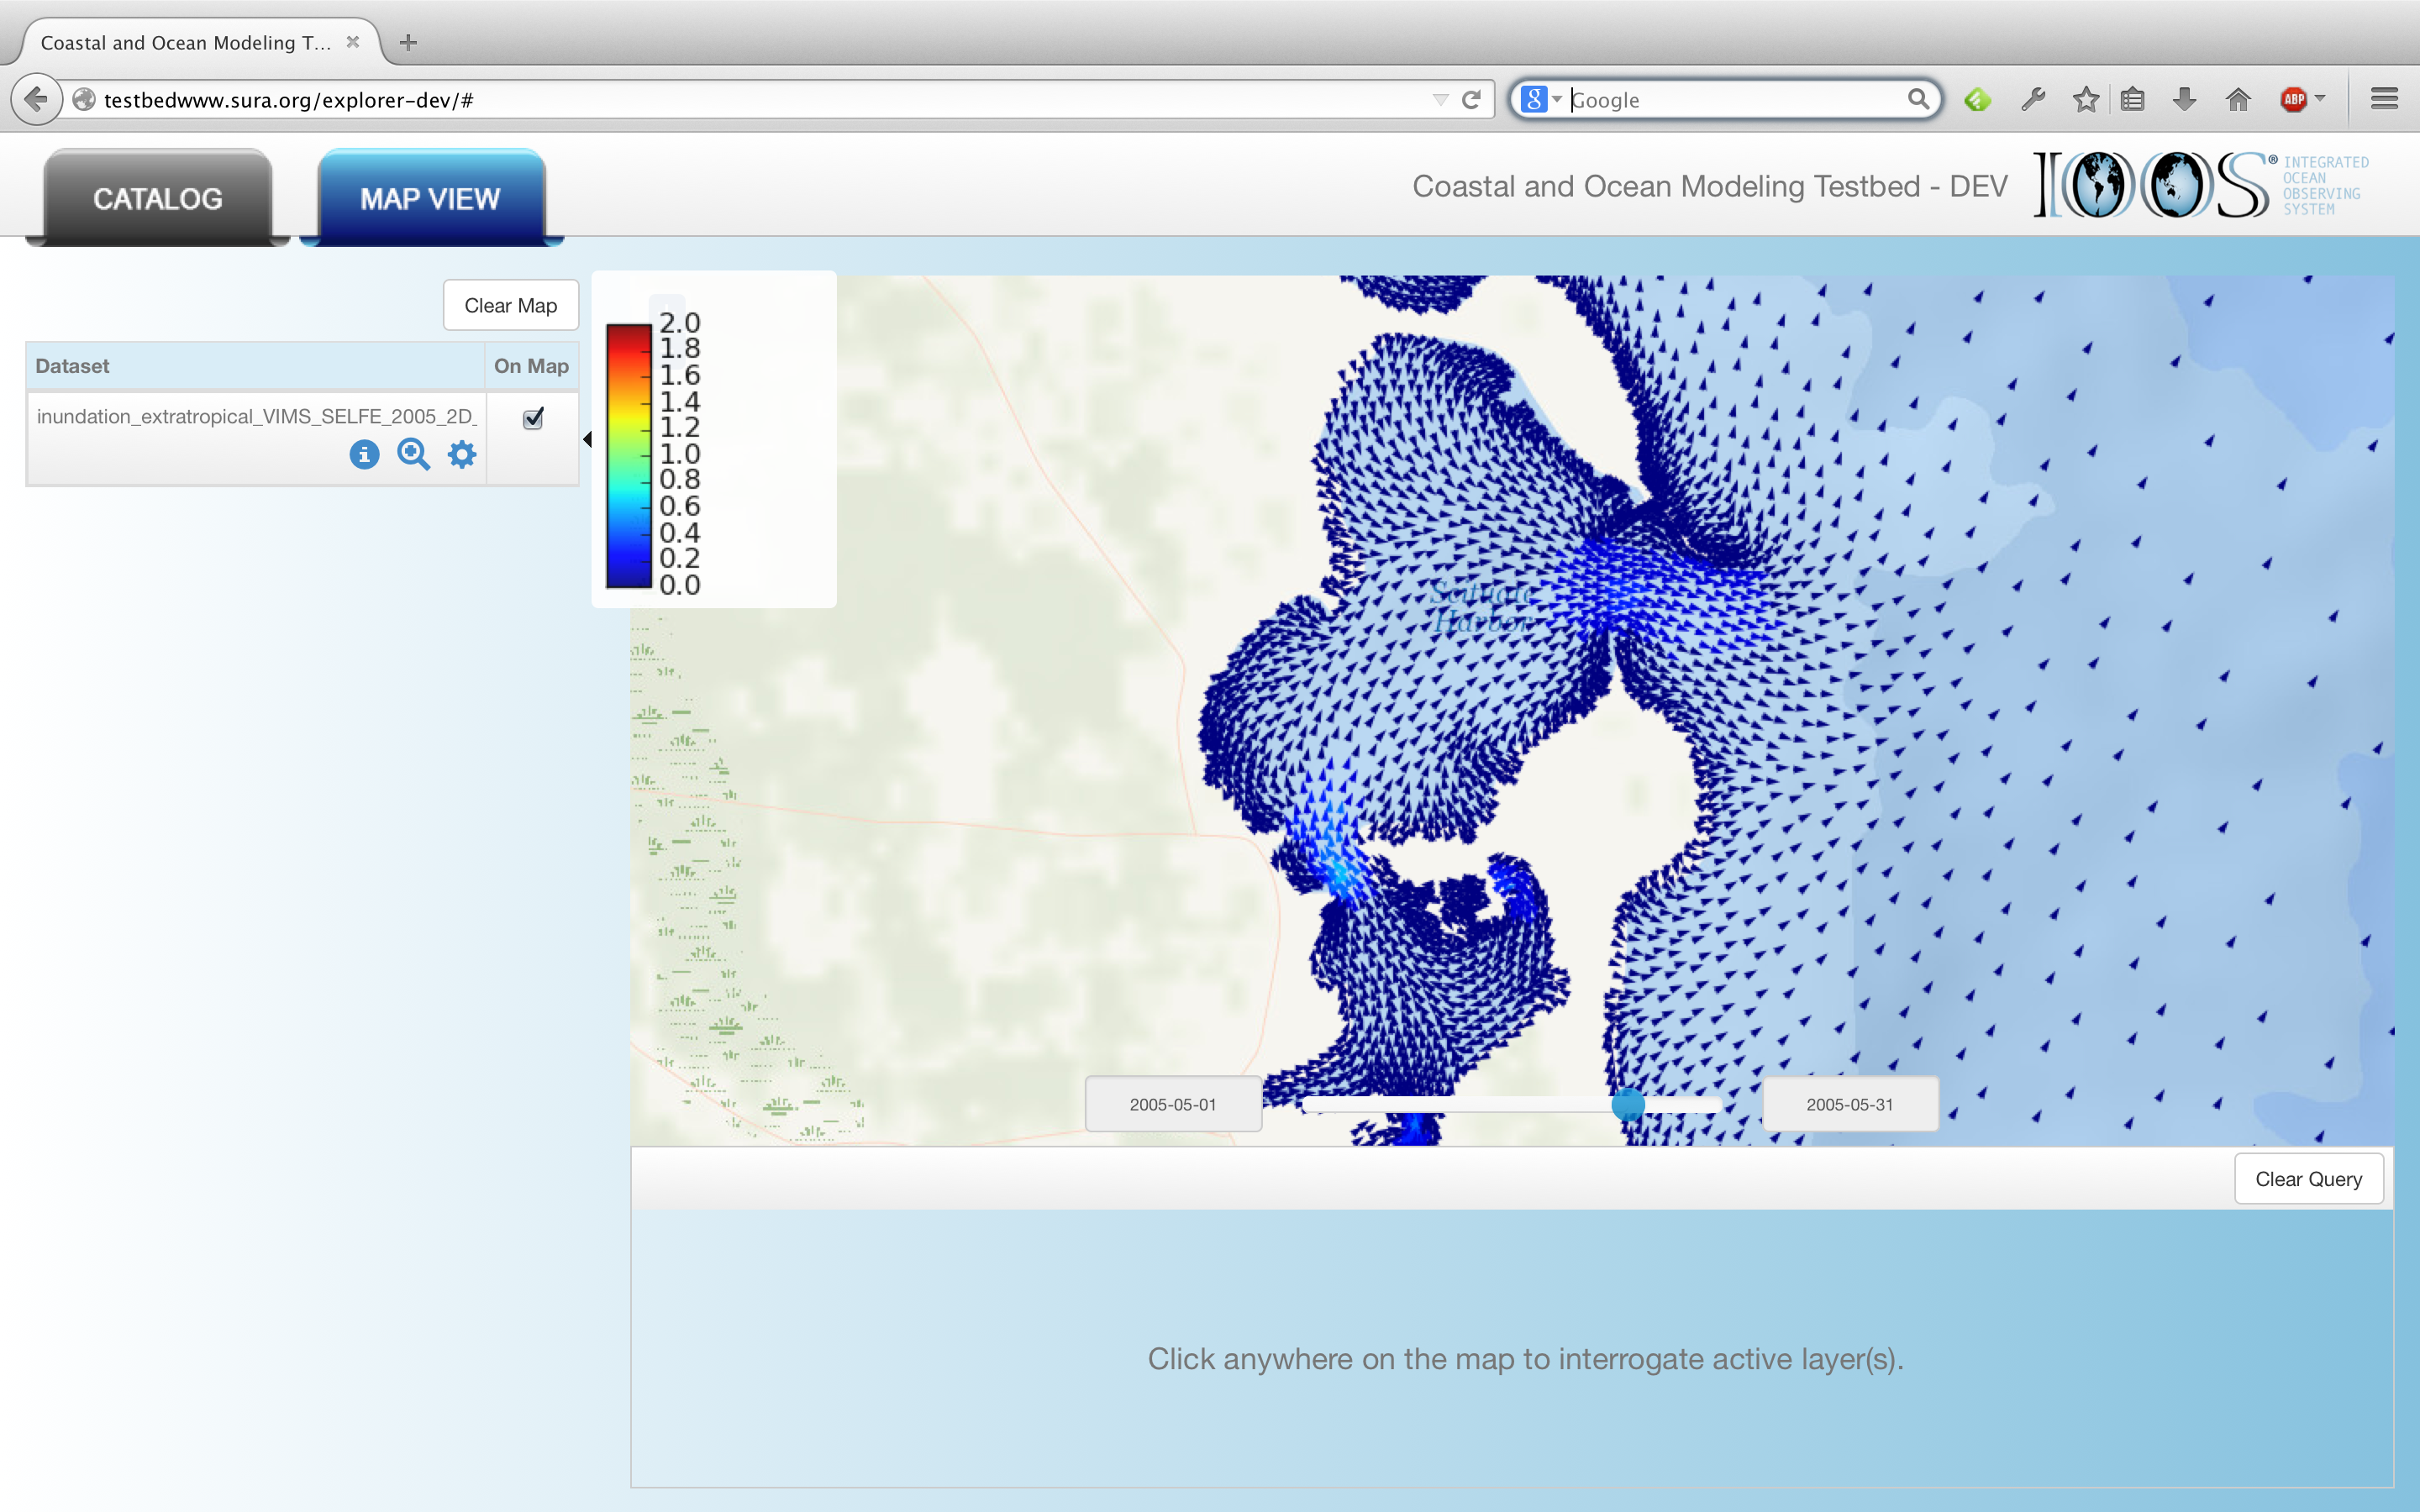
\includegraphics[width=\linewidth]{../figs/vims_selfe_ubaratropic_vbaratropic_chesapeake_bay}
  \textbf{Figure \getIncFigcounter{}}: \textit{SELFE model of current
    direction and speed in the Chesapeake Bay area.}
\end{minipage}
\figspace{}
\begin{minipage}[t]{\linewidth}
  \centering
  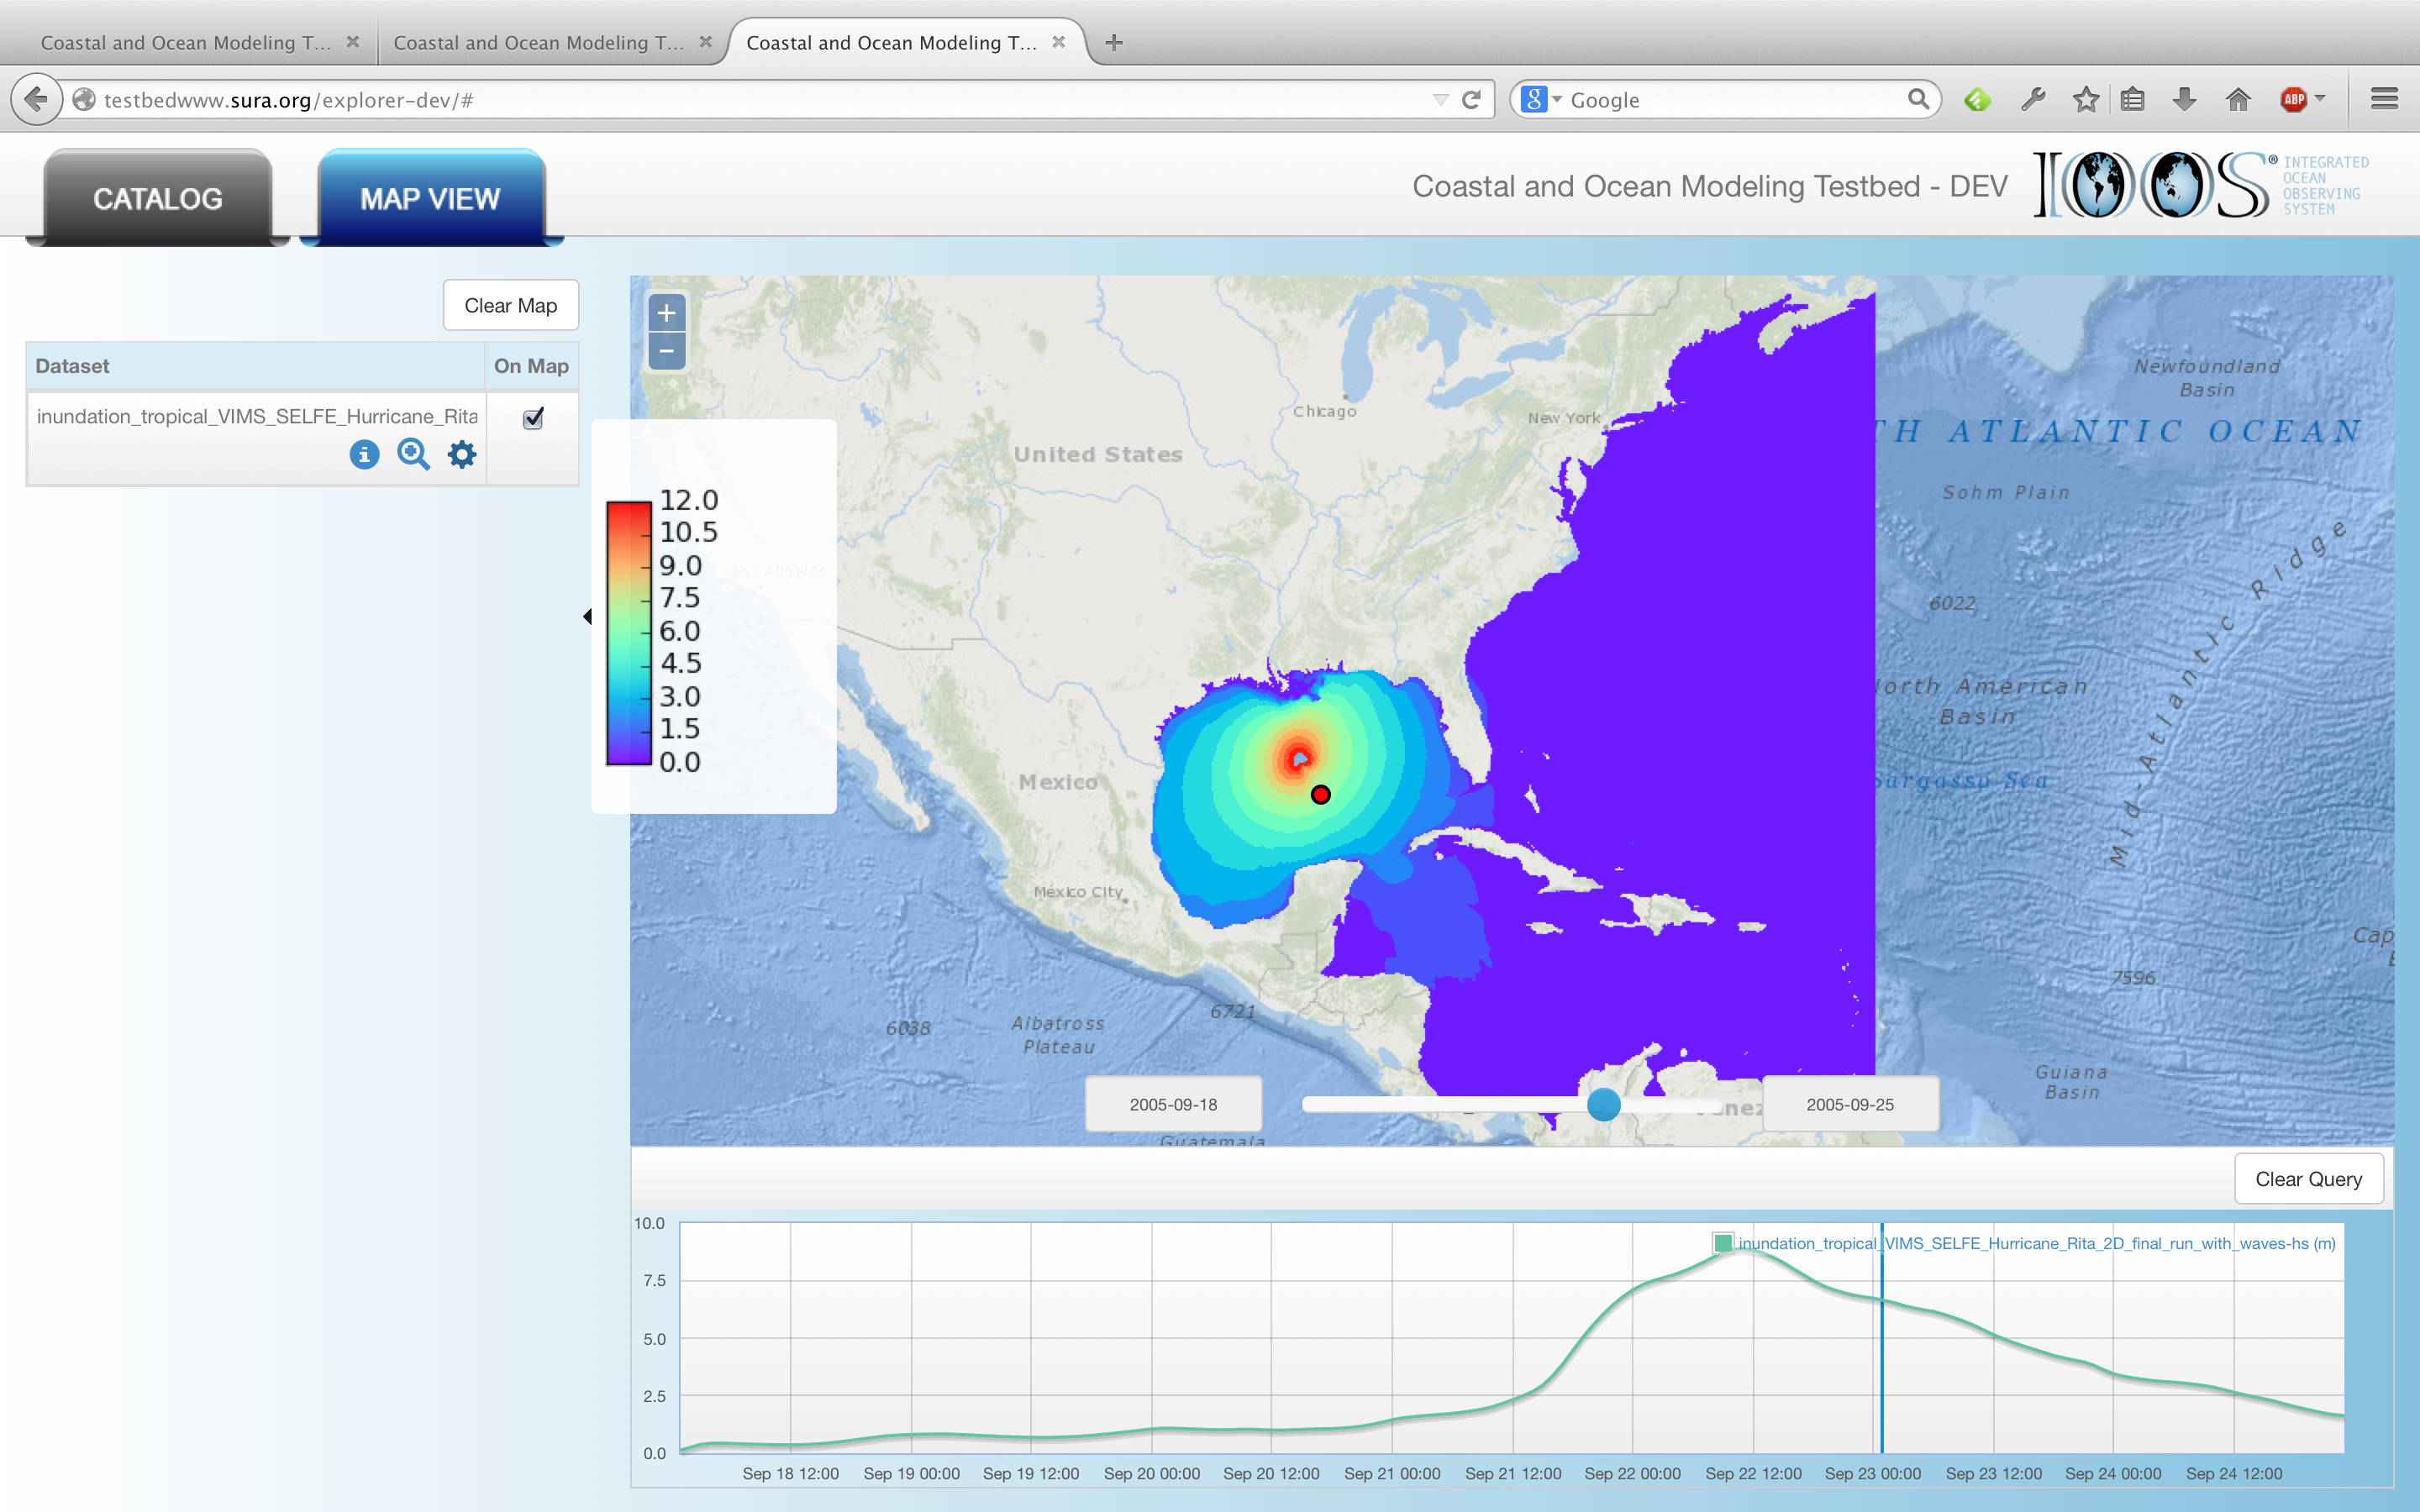
\includegraphics[width=\linewidth]{../figs/inundation_tropical_VIMS_SELFE_hurricane_rita_2d_final_run_with_waves_sea_surface_wave_significant_height}
  \textbf{Figure \getIncFigcounter{}}: \textit{Visualizing SELFE model of significant sea surface wave height along the eastern coast of the United States. The underlying topology is an unstructured grid with over 5 million nodes which SCI-WMS can handle in real time.}
\end{minipage}
\end{document}
